\documentclass{beamer}
\usetheme[white]{Wisconsin}
\usepackage{longtable}
\usepackage{graphicx}
\usepackage{listings}
\usepackage{color}
%% The amssymb package provides various useful mathematical symbols
\usepackage{amssymb}
%% The amsthm package provides extended theorem environments
\usepackage{amsthm} \usepackage{amsmath}
%% \usepackage{eqnarray}
\usepackage[mathcal]{euscript} \usepackage{color}
\usepackage{textcomp}
\usepackage{algorithm,algorithmic}
\usepackage[retainorgcmds]{IEEEtrantools}
\usepackage[absolute,overlay]{textpos}
  \setlength{\TPHorizModule}{1mm}
  \setlength{\TPVertModule}{1mm}
\definecolor{listinggray}{gray}{0.9}
\definecolor{lbcolor}{rgb}{0.9,0.9,0.9}
\lstset{
  backgroundcolor=\color{lbcolor},
  tabsize=4,
  rulecolor=,
  language=c++,
  basicstyle=\scriptsize,
  upquote=true,
  aboveskip={1.5\baselineskip},
  columns=fixed,
  showstringspaces=false,
  extendedchars=true,
  breaklines=true,
  prebreak =
  \raisebox{0ex}[0ex][0ex]{\ensuremath{\hookleftarrow}},
  frame=single,
  showtabs=false,
  showspaces=false,
  showstringspaces=false,
  identifierstyle=\ttfamily,
  keywordstyle=\color[rgb]{0,0,1},
  commentstyle=\color[rgb]{0.133,0.545,0.133},
  stringstyle=\color[rgb]{0.627,0.126,0.941},
}

%% colors
\setbeamercolor{boxheadcolor}{fg=white,bg=UWRed}
\setbeamercolor{boxbodycolor}{fg=black,bg=white}

%%----------------------------------------------------------------------------%%
\author{Luke J. Kersting
    \\ NEEP
    \\ University of Wisconsin - Madison
    \\ FRENSIE Meeting
}

\date{\today}
\title{Review of Summer at Sandia National Lab}
\begin{document}
\maketitle

%%----------------------------------------------------------------------------%%
\begin{frame}{Outline}

  \begin{itemize}
    \item Interaction at Sandia
    \item Condensed History's History
    \item Moment Preserving Method
    \item Adjoint Analog Transport
  \end{itemize}

\end{frame}

%%----------------------------------------------------------------------------%%
\begin{frame}{Sandia}

    \begin{figure}
     
\includegraphics[width=40mm]{twitter_logo.png}
   \end{figure}

\end{frame}

  %%----------------------------------------------------------------------------%%
  \begin{frame}{Condensed History Electron Transport}

  \begin{block}{Challenges}
    \begin{itemize}
      \item Electron charge increases scattering cross section
      \item Neutral Particles may scatter a couple dozen times over a distance
      \item Electrons may scatter 10,000 or more times over the same distance
      \item Purely analog transport is impractical at higher energies
      \item Approximations must be made to reduce computation costs
      \item Monte Carlo development lags behind
    \end{itemize}
  \end{block}
    
  \begin{block}{A “Condensed” Random Walk method was developed}
    \begin{itemize}
      \item Electrons are moved a set step length
      \item A multiply scattering theory is sampled to find the outgoing direction
      \item The Continuous Slowing Down Approximation (CSDA) is used to calculate energy loss
      \item Production of secondary are averaged
      \item Approximations don’t hold below 1 keV
      \item Uses infinite medium approximation
    \end{itemize}    
  \end{block}  

\end{frame}

%%----------------------------------------------------------------------------%%
\begin{frame}{Condensed History Step}
  
\begin{figure}[r]
  \centering
  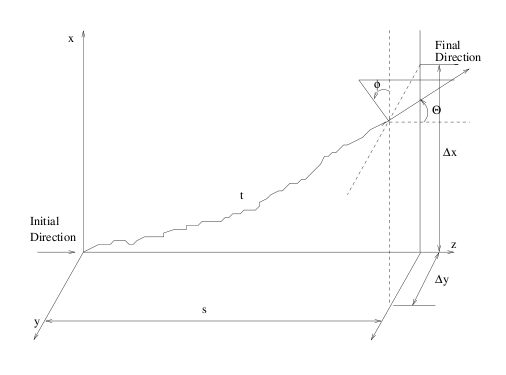
\includegraphics[width=90mm]{electron_step.png}
  \caption{Schematic of electron transport mechanics model in EGS. Where $s$ is the step length, $t$ the total distance traveled, $\Delta x$ and $\Delta y$ are the lateral displacements, $\Theta$ and $\phi$ are the final polar and azimuthal angles.}
\end{figure}

\end{frame}

  %%----------------------------------------------------------------------------%%
  \begin{frame}{Improvements to Condensed History}

  \begin{block}{Improving Transport Mechanics}

    \begin{itemize}
      \item Random Hinge transport 
      \item Modified Random Hinge transport
      \item More accurate Transport near boundaries
    \end{itemize}
  
  \end{block}
    
  \begin{block}{Mixed Analog/Condensed Simulation}
    \begin{itemize}
      \item Hard events involving large angle scattering, secondary particles, and
catastrophic interactions are analog
      \item Soft events involving small angle scattering are condensed
      \item Majority of electron cross section is due to soft elastic scattering
      \item Below 1 keV simulation becomes purely analog
    \end{itemize}    
  \end{block}  
    
    \begin{figure}
     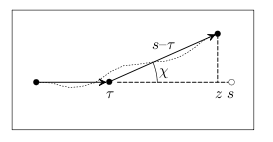
\includegraphics[width=40mm, x=-10cm]{random_hinge.png}
   \end{figure}
\end{frame}

%%----------------------------------------------------------------------------%%
  \begin{frame}{Moment Preserving Method (MP)}

  \begin{block}{Advantages}
    \begin{itemize}
      \item Legendre moments of the cross section are preserved
          \begin{itemize}
      \item mfps are reduced, increasing efficiency
      \item Less forward peaked angular scattering distribution
      \item Accuracy can be maintained by preserving some of the low-order moments
    \end{itemize}    
    
      \item Simplified physics that reflect the analog process are used
      \item Implementation simpler than Condensed History
      \item Distribution is no longer continuous but discrete

    \end{itemize}
  \end{block}


\end{frame}

  %%----------------------------------------------------------------------------%%
  
  \begin{frame}{Reduced Order Physics (ROP)}

  \begin{block}{The Boltzmann Collision Operator Approximated Using ROP}
    \begin{itemize}
      \item Integral form maintained
      \item Keeps correct transport mechanics
      \item Allows single-event simulations
    \end{itemize}    
      \end{block}
    
      \begin{block}{The analog cross section, $\Sigma$, is replaced with a ROP cross section,$\tilde{\Sigma}$ }
      $\tilde{\Sigma}$ preserves a finite number of moments of the analog cross section
      $$ \Sigma_{el,l}=2\pi\int_{-1}^{1}P_l(\mu)\Sigma_{el}(\mu)d\mu$$
      $$\tilde{\Sigma}_{el,l}=\Sigma_{el,l}  \text{   for  } l=1,2,..., L$$ 

  \end{block}


\end{frame}

  %%----------------------------------------------------------------------------%%
    \begin{frame}{ROP Elastic Cross Section}

  \begin{block}{MP Method Only}
        $$\tilde{\Sigma}(E,\mu) = \sum_{n=1}^{N}\frac{\alpha_n(E)}{2\pi}\delta[\mu-\zeta_n]+\frac{\alpha{N+1}(E)}{2\pi}\delta[\mu-1]$$
    \begin{itemize}
      \item Where $\alpha_n$ and $\zeta_n$ are the weights and nodes of the Radau quadrature
      \item The $\zeta_{N+1}=1$ node and weight are eliminated
    \end{itemize}    
      \end{block}
    
      \begin{block}{Hybrid Method}
      $$\tilde{\Sigma}(E,\mu) = \Sigma^{Analog}(E,\mu) +\sum_{n=1}^{N}\frac{\alpha_n(E)}{2\pi}\delta[\mu-\zeta_n]$$
          \begin{itemize}
      \item Below a cutoff, $\mu*$, analog transport is used
      \item Where $ \Sigma^{Analog}(E,\mu)$ is the analog cross section for $\mu \in  [-1, \mu*)$
      \item Only have discrete angles above $\mu*$
    \end{itemize}    

  \end{block}


\end{frame}


%%----------------------------------------------------------------------------%%
\begin{frame}{Adjoint Transport}

%\begin{block}{Time-Independent Boltzmann Equation}
%\begin{multline}
%  -\Omega \nabla \phi^{\dagger}(\boldsymbol r,E,\boldsymbol\Omega) + 
%  \Sigma_t(\boldsymbol{r},E)\phi^{\dagger}(\boldsymbol{r},E,\boldsymbol{\Omega}) = \\
%  \int\int\Sigma_t(\boldsymbol{r},E)C(\boldsymbol{r},E\rightarrow E',\boldsymbol{\Omega}\rightarrow\boldsymbol{\Omega})\phi^{\dagger}(\boldsymbol{r},E',\boldsymbol{\Omega})dE'd\Omega' + 
%  D(\boldsymbol{r},E,\boldsymbol{\Omega})
%\end{multline}
%\end{block}

\begin{block}{Adjoint Collision Kernel}
\begin{multline}
C^{\dagger}(\boldsymbol{r'},E'\rightarrow E,\boldsymbol{\Omega'}\rightarrow\boldsymbol{\Omega}) = \\
\sum_A p_A^{\dagger}(\boldsymbol{r'},E') \sum_j p^{\dagger}_{j,A}(E') \frac{\sigma_{j,A}(E)c_{j,A}(E)f_{j,A}(E\rightarrow E',\boldsymbol{\Omega}\rightarrow\boldsymbol{\Omega'})}{\sigma^{\dagger}_{j,A}(E')}
\end{multline}

\begin{equation}
\sigma^{\dagger}_{j,A}(E') = \int\sigma_{j,A}(E)c_{j,A}(E)f_{j,A}(E\rightarrow E')dE
\end{equation}

\begin{equation}
p^{\dagger}_A(\boldsymbol{r'},E') = \frac{\Sigma^{\dagger}_A(\boldsymbol{r'},E')}{\Sigma{\dagger}(\boldsymbol{r'},E')}
~~~~~~~~~~~~~~~~~~
p^{\dagger}_{j,A}(E') = \frac{\sigma^{\dagger}_{j,A}(E')}{\sigma^{\dagger}_A(E')} \nonumber
\end{equation}

\end{block}

\end{frame}

%%----------------------------------------------------------------------------%%
\begin{frame}{Adjoint Transport}

First the type of nuclide that the electron interacts with is sampled from:
\begin{equation}
p^{\dagger}_A(\boldsymbol{r'},E') = \frac{\Sigma^{\dagger}_A(\boldsymbol{r'},E')}{\Sigma{\dagger}(\boldsymbol{r'},E')}
\end{equation}

Then the reaction type is sampled from:
\begin{equation}
p^{\dagger}_{j,A}(E') = \frac{\sigma^{\dagger}_{j,A}(E')}{\sigma^{\dagger}_A(E')} \nonumber
\end{equation}

Finally, $E$ and $\Omega$ are sampled from:
\begin{equation}
f^{\dagger}_{j,A}(E'\rightarrow E,\boldsymbol{\Omega'}\rightarrow\boldsymbol{\Omega}) = 
\frac{\sigma_{j,A}(E)c_{j,A}(E)f_{j,A}(E\rightarrow E',\boldsymbol{\Omega}\rightarrow\boldsymbol{\Omega'})}{\sigma^{\dagger}_{j,A}(E')} \nonumber
\end{equation}

\end{frame}


%%----------------------------------------------------------------------------%%
\begin{frame}{Adjoint Cross-Sections}
Electrons reactions are not specifically dependent on the incoming and outgoing angle, 
but instead on $\mu$. Therefore the equations reduced to:
\begin{equation}
\sigma^{\dagger}(E') = \int\int\sigma(E)c(E)f(E \rightarrow E', \mu)dEd\mu
\end{equation}

\begin{equation}
f^{\dagger}(E' \rightarrow E, \mu) = \frac{\sigma(E)c(E)f(E \rightarrow E', \mu)}{\sigma^{\dagger}(E')}
\end{equation}

\begin{equation}
\sigma^{\dagger}(E' \rightarrow E, \mu) = \sigma(E \rightarrow E', \mu)
\end{equation}

\end{frame}

  %%----------------------------------------------------------------------------%%
    \begin{frame}{Atomic Excitation}

  \begin{block}{An incident electron loses some energy by exciting an outer electron to higher energy states}
    \begin{itemize}
      \item There is no angular deflection (interaction is considered distant)
      \item There are no secondary particles
      \item Energy loss to incident electron
    \end{itemize}
  \end{block}
  
    \begin{figure}
     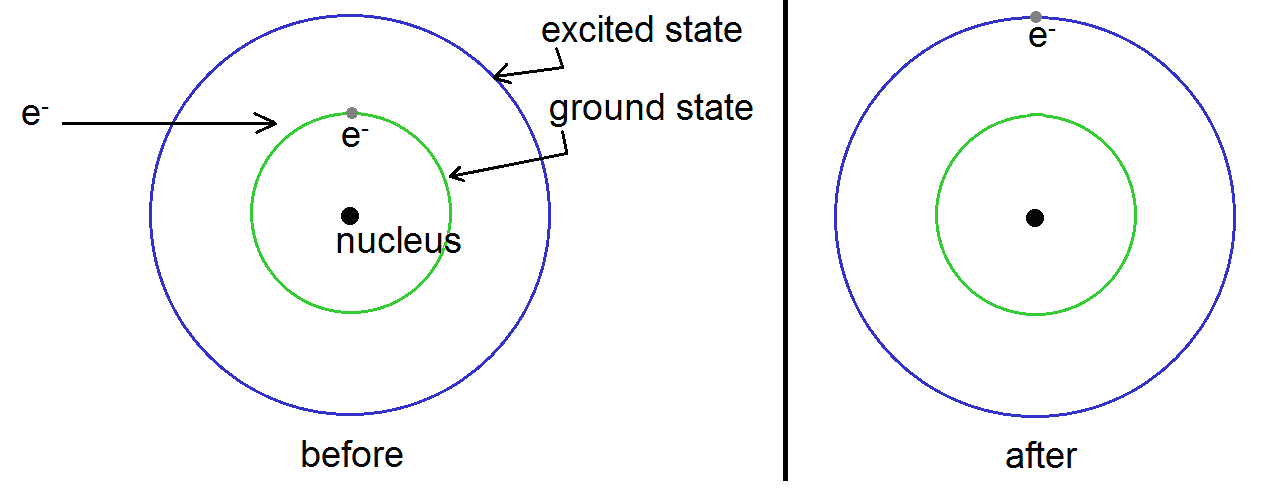
\includegraphics[width=80mm]{excitation.png}
   \end{figure}

\end{frame}

%%----------------------------------------------------------------------------%%
\begin{frame}{Atomic Excitation}
	\begin{itemize}
	\item Their is no angular deflection
	\item Cross-sections are independent of angle
	\item Each incoming energy will scatter into a unique outgoing energy
	\item There is a one-to-one correspondence between the incoming and outgoing energy
	\end{itemize}

\begin{align}
\sigma^{\dagger}(E' \rightarrow E, \mu) = &\sigma(E \rightarrow E', \mu) = \nonumber \\
\sigma^{\dagger}(E') = &\sigma(E)
\end{align}

\begin{equation}
f^{\dagger}(E', \mu) = \frac{\sigma(E)f(E, \mu)}{\sigma^{\dagger}(E')} = f(E, \mu)
\end{equation}

\end{frame}

  %%----------------------------------------------------------------------------%%
    \begin{frame}{Electroionization}

  \begin{block}{An incident electron scatters off an atom, ionizing an electron from one of its subshells}
    \begin{itemize}
      \item A subshell is directly sampled
      \item A knock-on electron is ejected
      \item The incident electron energy is reduced by $E_{Knock} + E_{Binding}$
    \end{itemize}
  \end{block}
  
      \begin{figure}
     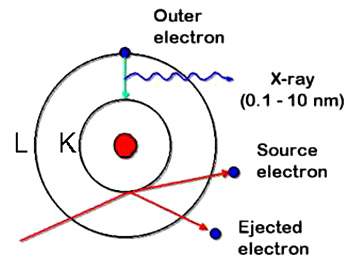
\includegraphics[width=50mm]{Inner_Shell_Ionization.jpg}
   \end{figure}

\end{frame}

%%----------------------------------------------------------------------------%%
\begin{frame}{Electroionization}
	\begin{itemize}
	\item A second electron is produced
	\item There is a unique angle for each $E \rightarrow E'$ pair
	\end{itemize}

\begin{equation}
p(E \rightarrow E', \mu) = f(E \rightarrow E')
\end{equation}

\begin{equation}
\sigma^{\dagger}(E') = \int\sigma(E)f(E \rightarrow E')dE
\end{equation}

\begin{equation}
f^{\dagger}(E'\rightarrow E, \mu) = \frac{\sigma(E)f(E \rightarrow E')}{\sigma^{\dagger}(E')} 
\end{equation}

\end{frame}

  %%----------------------------------------------------------------------------%%
    \begin{frame}{Bremsstrahlung}

  \begin{block}{An incident electron interacts with an atom releasing electromagnetic radiation}
    \begin{itemize}
      \item A photon is ejected
      \item Incident electron energy is reduced by $E_{\gamma}$
      \item The incident electron energy is reduced by $E_{Knock} + E_{Binding}$
    \end{itemize}
  \end{block}
  
      \begin{figure}
     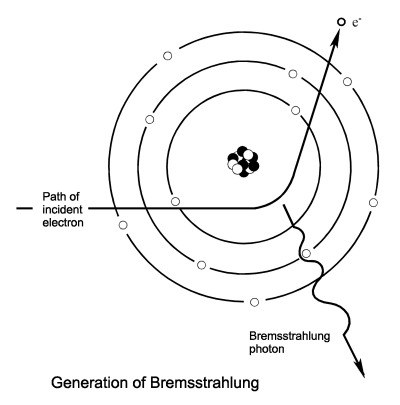
\includegraphics[width=50mm]{brem.png}
   \end{figure}


\end{frame}

%%----------------------------------------------------------------------------%%
\begin{frame}{Bremsstrahlung}
	\begin{itemize}
	\item Angular deflection is assumed to be negligible
	\item Cross-sections are independent of angle
	\end{itemize}

\begin{align}
\sigma^{\dagger}(E' \rightarrow E, \mu) = & \sigma(E \rightarrow E', \mu) =\nonumber \\
\sigma^{\dagger}(E' \rightarrow E) = & \sigma(E \rightarrow E') = \sigma(E)f(E \rightarrow E')
\end{align}

\begin{equation}
\sigma^{\dagger}(E') = \int\sigma(E)f(E \rightarrow E')dE
\end{equation}

\begin{equation}
f^{\dagger}(E' \rightarrow E) = \frac{\sigma(E)f(E \rightarrow E')}{\sigma^{\dagger}(E')}
\end{equation}


\end{frame}

  %%----------------------------------------------------------------------------%%   
  \begin{frame}{Elastic Scattering}

  \begin{block}{An incident electron scatters off a nucleus retaining its energy}
    \begin{itemize}
      \item Energy loss is assumed to be negligible
      \item There are no secondary particles
      \item Angular deflection occurs
    \end{itemize}
  \end{block}
  
      \begin{figure}
     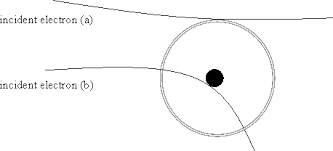
\includegraphics[width=60mm]{elastic2.png}
   \end{figure}

\end{frame}

%%----------------------------------------------------------------------------%%
\begin{frame}{Elastic Scattering}
	\begin{itemize}
	\item Their is no energy loss ($ E = E'$)
	\item Adjoint and Forward transport will be exactly the same
	\end{itemize}
\begin{align}
\sigma^{\dagger}(E' \rightarrow E, \mu) = &\sigma(E \rightarrow E', \mu) = \nonumber \\
\sigma^{\dagger}(E, \mu) = &\sigma(E, \mu)
\end{align}

Therefore equations $(6)$ and $(7)$ reduce to:
\begin{equation}
\sigma^{\dagger}(E') = \sigma(E)
\end{equation}

\begin{equation}
f^{\dagger}(E, \mu) = f(E, \mu)
\end{equation}

\end{frame}

  %%----------------------------------------------------------------------------%%
  
\end{document}